%
%  Chapter:  1 - Introduction
%  Modified: 2/16/2015
%  Author:   James Till Matta
%
%%%%%%%%%%%%%%%%%%%%%%%%%%%%%%%%%%%%%%%%%%%%%%%%%%%%%%%%%%

\chapter{INTRODUCTION}
\label{chp:intro}
\section{Rotation of Deformed Nuclei}
\label{sec:intro-rot-def-nuc}
Rotation is a universal phenomenon. It exists in the macroscopic world where objects can rotate independently about any set of axes. In the microscopic world of quantum mechanics, the situation is more complicated. Rotation about an axis of symmetry is forbidden since the wave function is unchanged. Rotation must be about an axis that is not an axis of symmetry; thus limiting it to objects that are deformed, \emph{i.e.} not spherical.

\subsection{Axial Deformation}
\label{ssec:intro-rot-axial-def}
Spherical nuclei are in many ways, exceptional; as Fig. \ref{fig:chp1-quad-def} shows, deformation occurs in many regions of the nuclear chart. Near closed shells, the deformation is slight enough that spherical models can be employed to describe most nuclear properties. However, further from magic numbers, there are regions of the nuclear chart where the deformation grows large enough that it can no longer be ignored. Examples of these regions are the $A\sim{}130$ region and the $A\sim{}160$ region.

\begin{figure}[t!]
\centerline{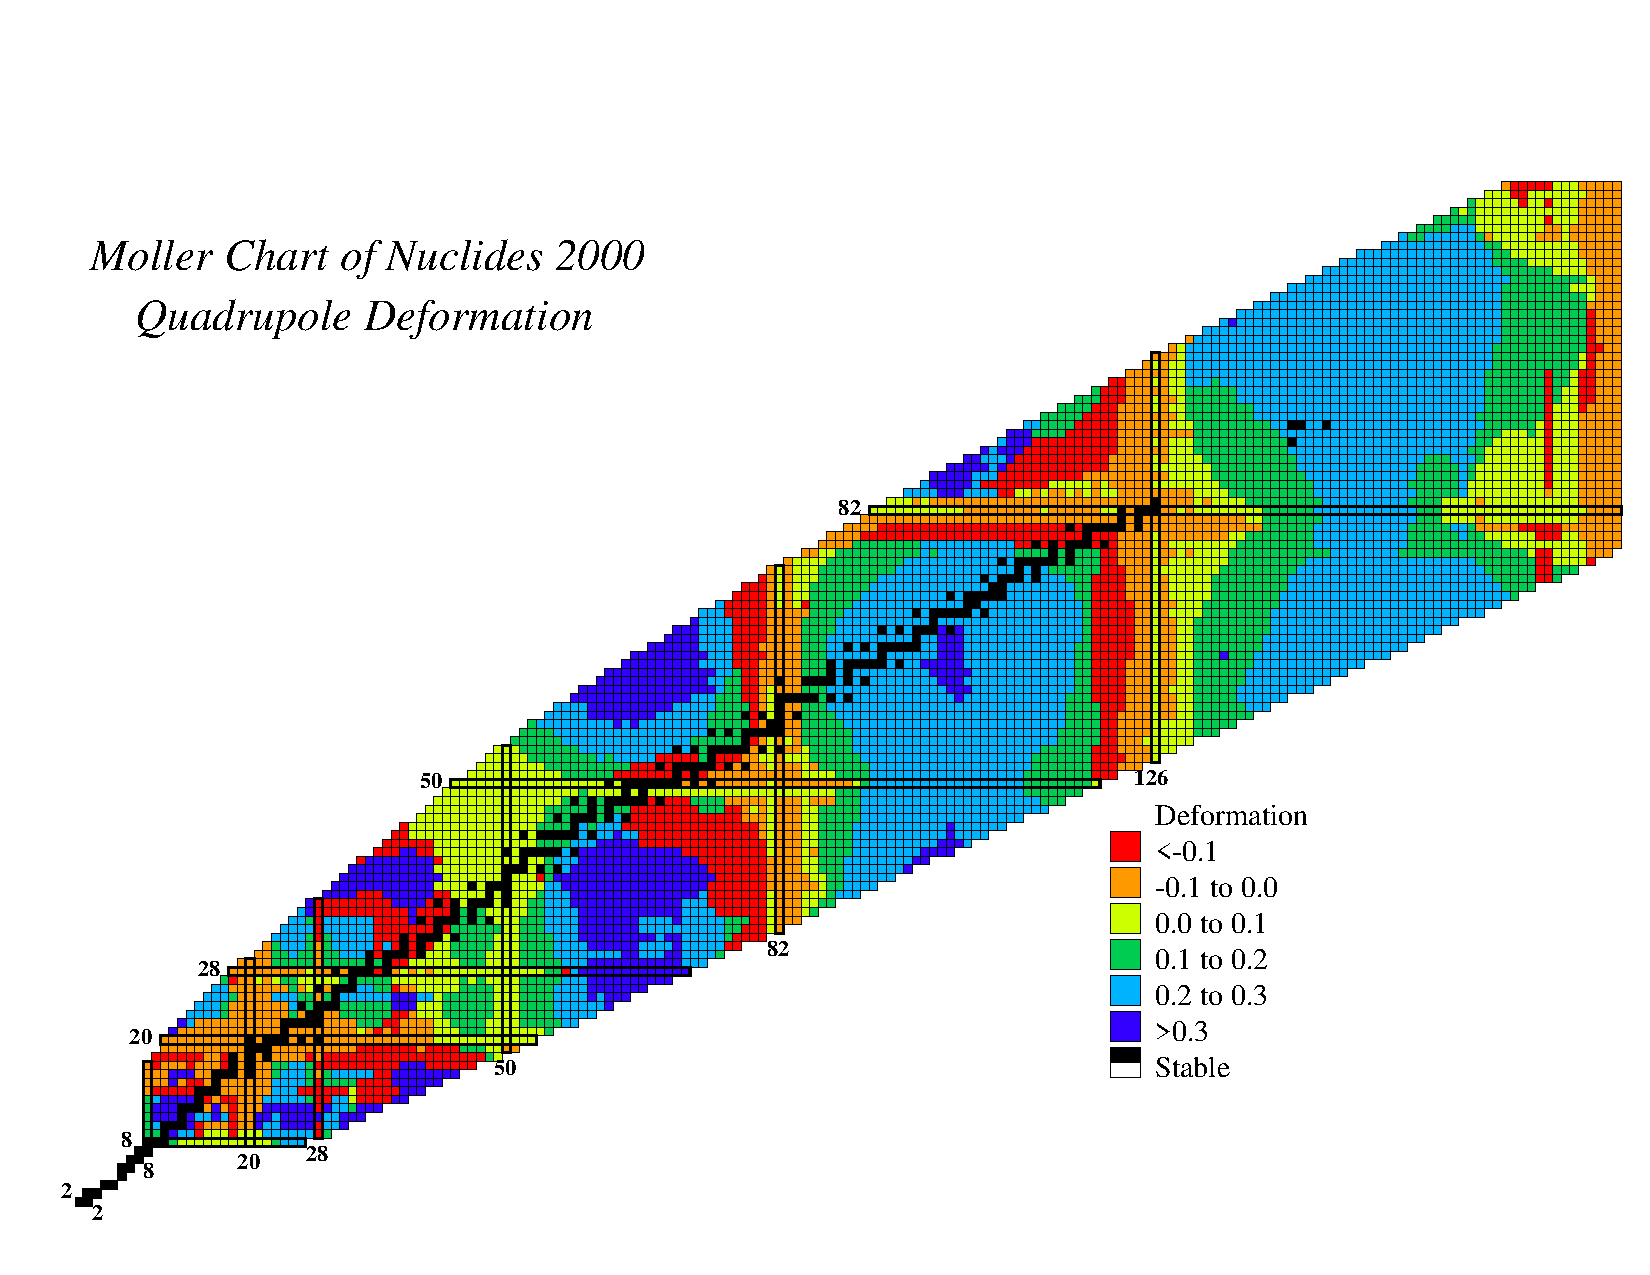
\includegraphics[width=\textwidth,clip=true,trim=0 0 0 75]{./img/c1/chart_thb2.pdf}}
	\caption{Quadrupole deformation parameter $\beta_2$ across the nuclear chart. Plot adapted from \cite{nilssonDiagrams} which used data from \cite{mollerGroundStateDef}.\label{fig:chp1-quad-def}}
\end{figure}

While axial symmetry includes both oblate (doorknob shaped) and prolate (cigar like) shapes, there are few oblate nuclei. The majority have prolate deformation. This is usually understood as an effect of single particle structure from the Nilsson model (the Nilsson model is discussed in more detail in Chapter 2). Overall, prolate deformation moves more orbitals to low energy than oblate deformation. Therefore in situations where there are several particles, a sum over these particles will favor prolate shapes.

\subsection{Triaxiality}
\label{ssec:intro-rot-triax}
Nuclear triaxiality has been a subject of interest for years. While most deformed nuclei are axial in their shape, triaxial shapes have been predicted at low to moderate spin for a few regions of the nuclear chart, \emph{e.g.} Z$\sim{}$60, N$\sim{}$76 and Z$\sim{}$46, N$\sim{}$66 \cite{groundStateTriax}. Triaxial shapes also occur in the Z$\sim{}$70, N$\sim{}$90 region, but are found in triaxial superdeformed bands at high spins. In searching for triaxiality we are aided by the existence of two unique fingerprints, chirality and wobbling; phenomena that cannot exist unless the nuclear shape is triaxial. Thus observation of either of these modes is important as they constitute irrefutable evidence of triaxiality.

%A third fingerprint, though not unique, signature inversion.

%\subsubsection{Signature Inversion}
%\label{sssec:intro-rot-sig-inversion}
%As will be discussed in section \ref{sssec:models-tac-pac}, principal axis solutions of the Tilted Axis Cranking model can be characterized by the signature quantum number $\alpha$. There are then two bands of states whose spin follows the selection rule in Eqn. \ref{eqn:chp2=TAC-PAC-spin-sel-rule} that have some energy splitting. Experimentally it has been observed that in some cases, this energy splitting inverts, and the unfavored signature becomes energetically favorable. Ref. \cite{sigInversionFingerprint} posits that this can only occur in nucleus with triaxial shape.  However Ref. \cite{sigInversionFromCrossing} shows that band crossing can cause it as well. This suggests there are two possible mechanisms

\subsubsection{Chirality}
\label{sssec:intro-rot-chiral}
First predicted in 1997  by S. Frauendorf and J. Meng, chirality occurs when the axis of rotation lies outside the plains spanned by the principal axes of the nucleus \cite{frauendorfChirality,chiralityOfNuclearRotation,frauendorfTAC}. Here a particle-like quasiparticle couples to the short axis, a hole-like quasi-particle couples to the long axis, and the triaxial rotor core rotates about the intermediate axis. In this configuration the total angular momentum points away from any of the principal planes of the nucleus and the three components of the angular momentum form a screw with respect to the total \cite{frauendorfChirality}.  When this configuration is present, the time-reversal symmetry of the nuclear wave function is broken and two nearly degenerate $\Delta{}I=1$ bands with similar electromagnetic properties emerge. Experiments have confirmed the existence of pairs of chiral bands in the $A\sim{}190$, $A\sim{}130$, $A\sim{}100$, and  $A\sim{}80$ regions of the chart of the isotopes; an example from each mass region can be found in Refs. \cite{chiralityMore135Nd,chiralityIn104Rh,chiralityIn188Ir,chiralityIn80Br}

\subsubsection{Wobbling}
\label{sssec:intro-rot-wob}
Of the two fingerprints of nuclear triaxiality, nuclear wobbling was perhaps the longest anticipated. First predicted by A. Bohr and B. Mottelson in Ref. \cite{bohrMottelson2}, wobbling was not observed until the work in 2001 by \O{}deg\aa{}rd \emph{et al.} \cite{wobblingIn163Lu}. Later four more wobbling nuclei were discovered, expanding the list to $^{161,163,165,167}$Lu and $^{167}$Ta \cite{wobblingIn163Lu,wobblingIn163LuTwoPhonon,wobblingIn165Lu,wobblingIn167Lu,wobblingIn161Lu,wobblingIn167Ta}. The wobbling mode is the quantum mechanical analog of the spinning motion of an asymmetric top. In the high spin limit the wobbling mode is a harmonic vibration describing oscillation of a principal axis of the nucleus about the angular momentum vector.

Understanding of the wobbling mode in nuclei has evolved quickly over the last 15 years. Bohr and Mottelson first showed that a rotating nucleus with stable triaxial deformation could have its rotational angular momentum precess and nutate about the principal axis of a nucleus \cite{bohrMottelson2} (in analogy to the classical asymmetric top) quite some time ago. In 1995, Schnack-Petersen \emph{et al.} suggested that bands in $^{163,165}$Lu which are based on the $\pi{}(i_{13/2})$ configuration, occupied a triaxial superdeformed (TSD) minimum of the total Routhian surface \cite{tsdLutetium}. Following this there was a rush of wobbling discoveries in $^{161,163,165,167}$Lu from 2001 to 2005 \cite{wobblingIn163Lu,wobblingIn163LuTwoPhonon,wobblingIn165Lu,wobblingIn167Lu,wobblingIn161Lu}. Further searches conducted in the region on $^{171}$Ta \cite{wobbSearch171Ta}, $^{169}$Ta \cite{wobbSearch169Ta}, $^{163}$Tm \cite{wobbSearch163Tm}, $^{171,172}$Hf \cite{wobbSearch1712Hf}, and $^{160,161}$Tm \cite{wobbSearch1601Tm} yielded no further wobbling bands. This left an open problem as to why wobbling was only appearing in the Lu isotopes.

A possible solution to this problem was offered up in the Tilted Axis Cranking calculations by Frauendorf, presented in Ref. \cite{wobbSearch163Tm}. The calculations suggest that the Lu TSD minima have a low density of states; low enough that the relatively high excitation energy wobbling mode can be observed. Contrariwise, the TSD minima of other nuclei in the region had a high density of states which could produce many different TSD bands with alternate configurations at similar energies. Thus, it is not that wobbling is absent in nuclei that are not Lu isotopes, but instead, that outside of the Lu isoptopes there was a competition between wobbling and particle hole excitations that favored the latter. This result motivated a search of $^{167}$Ta for wobbling which in 2009 yielded the first wobbling band outside the Lu isotopes \cite{wobblingIn167Ta}.

\subsubsection{Triaxiality in the A$\sim{}130$ Region}
\label{sec:trw-triax}
As previously stated Ref. \cite{groundStateTriax} predicts the region around $Z\sim{}60$ and $N\sim{}76$ to have triaxial shapes at low to moderate spin. The prevalence of triaxial shapes in this region is confirmed by the numerous observations of chirality \cite{chiralityIn134Pr,chiralityA130Region,chiralityUpperA130Region,chiralityA130Region2,chirality136Pm,chiralityMore135Nd,chiralityIn135Nd,chiralityMulti133Cs}. Additionally, a more exotic and stable chirality was identified in \cite{chiralityMore135Nd,chiralityIn135Nd} and confirmed via lifetime measurement to extract the $B(M1)$ and $B(E2)$ values of the partner bands to ensure that they are the same \cite{chiralityIn135Nd}. In fact, in this case, a transition from the more usual chiral vibration (where the angular momentum vector oscillates in a plane perpendicular to the axes the quasiparticles are coupled to) to static chirality where this oscillation slows to nearly stationary resulting in the bands becoming quite close to degenerate.

With this demonstration that triaxiality is rampant in the A$\sim{}130$ region, it becomes logical to set one's sights on that as the next region to search for wobbling. 

\section{Previous Cases of Wobbling}
\label{sec:trw-prev}
The wobbling bands of the previously known wobblers are pictured in Figs. \ref{fig:chp1-first-wobb}, \ref{fig:chp1-second-wobb}, and \ref{fig:chp1-last-wobb}). These figures are in chronological order of discovery from left to right, top to bottom.%The wobbling bands of $^{163}$Lu \cite{wobblingIn163Lu} and  $^{165}$Lu \cite{wobblingIn165Lu} are pictured in the left and right panels of Fig. \ref{fig:chp4-first-wobb}. The wobbling bands in $^{167}$ \cite{wobblingIn167Lu} and  $^{161}$Lu \cite{wobblingIn161Lu} are pictured in the left and right panels of Fig. \ref{fig:chp4-second-wobb}. The wobbling bands of the last of the wobblers known prior to this work, $^{167}$Ta, is in Fig. \ref{fig:chp4-last-wobb}). 

\begin{figure}[ht!]
\centerline{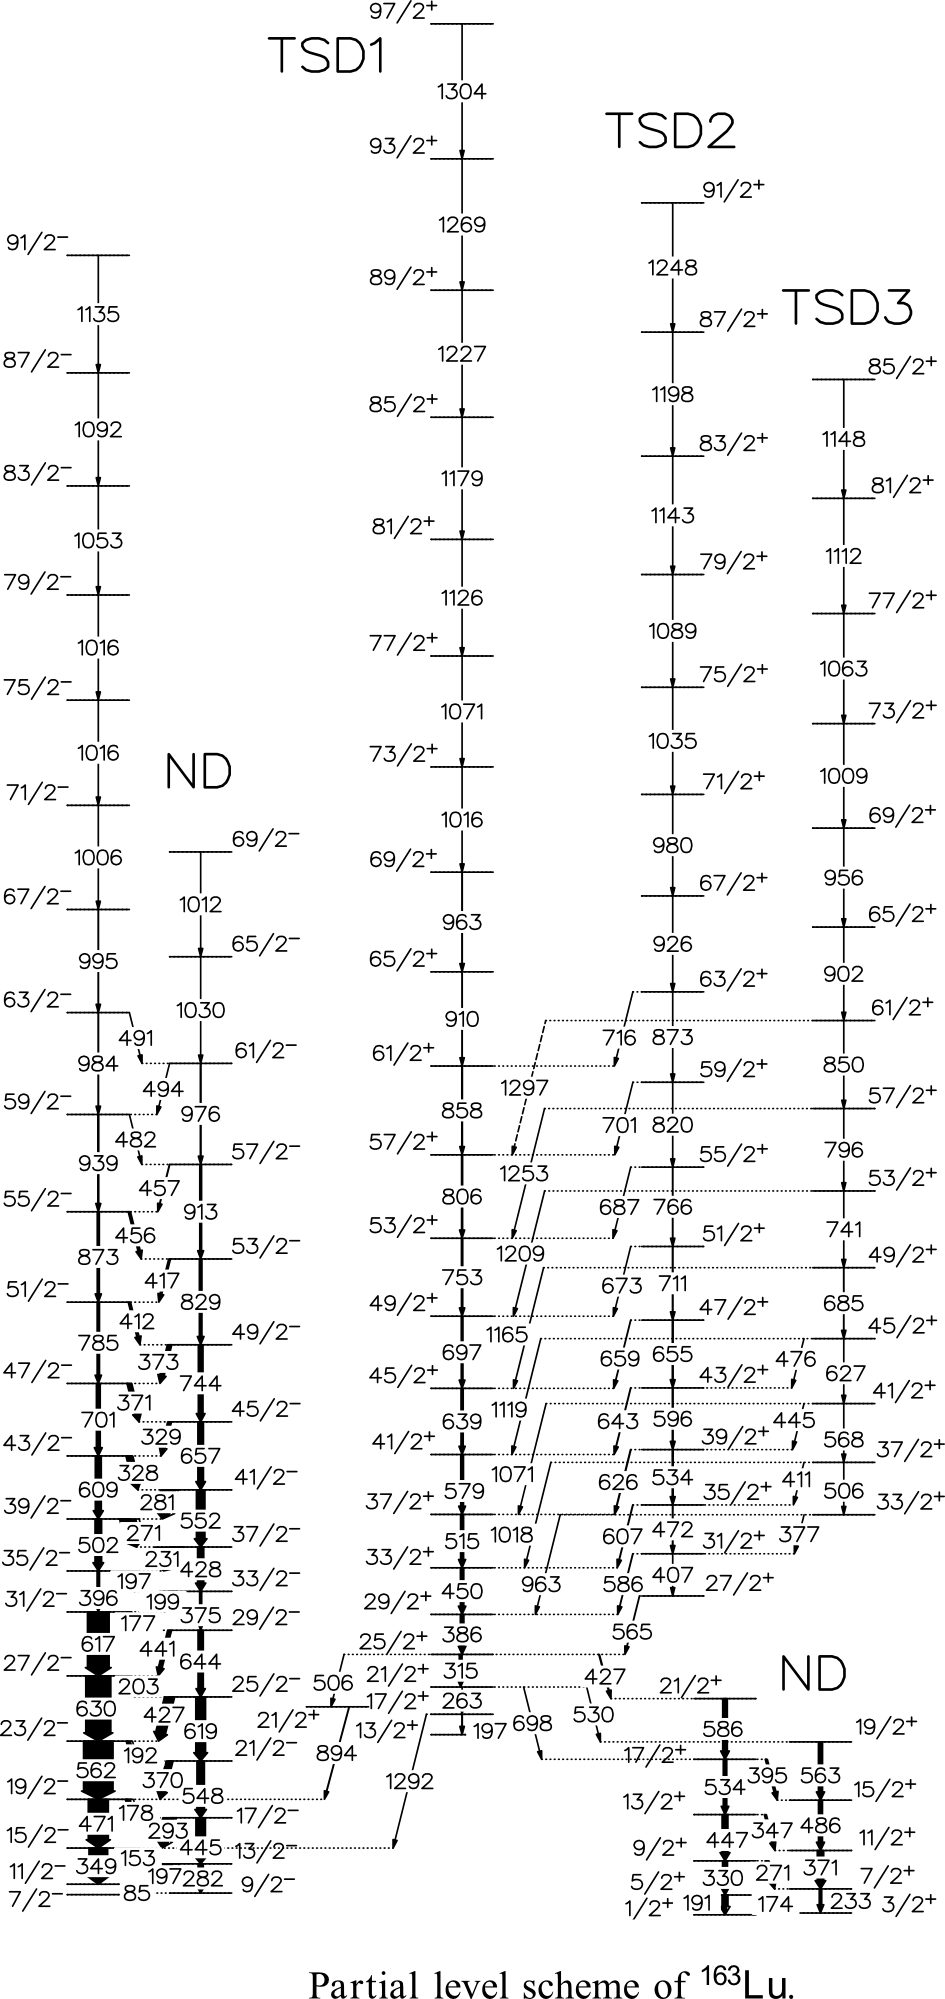
\includegraphics[width=0.4\textwidth]{./img/c1/163Lu_scheme.png}\hspace{0.1\textwidth}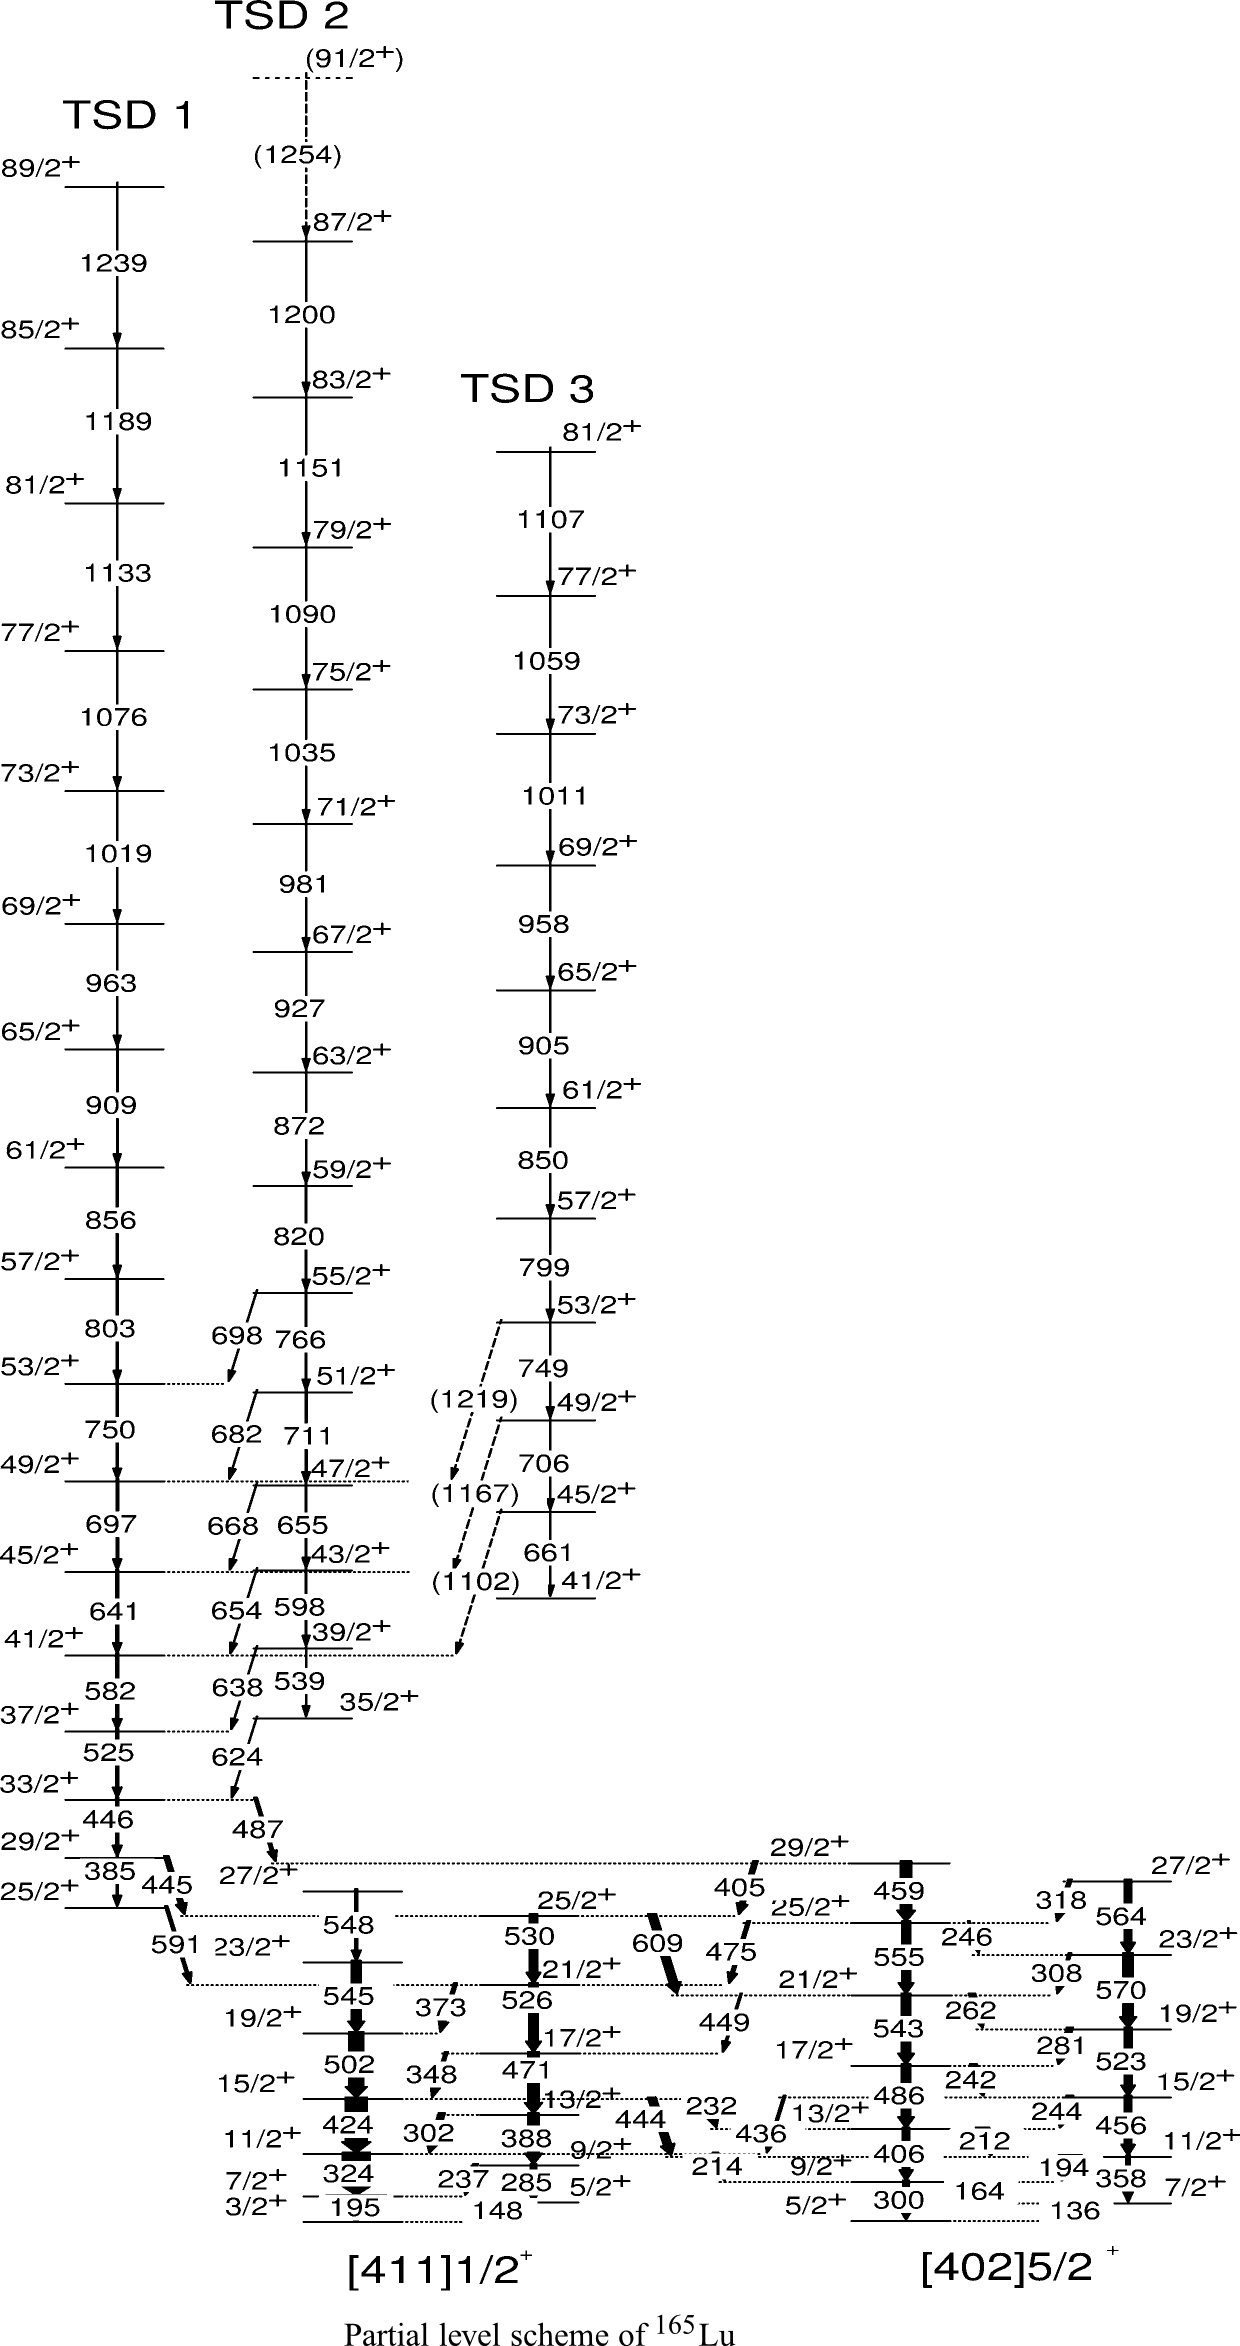
\includegraphics[width=0.4\textwidth]{./img/c1/165Lu_scheme.png}}
	\caption{Partial level schemes of $^{163}$Lu (left) and $^{165}$Lu (right). Figures adapted from Ref. \cite{wobblingIn163LuTwoPhonon} and Ref. \cite{wobblingIn165Lu}, respectively. In $^{163}$Lu the $n_w=0,1,2$ bands are labeled TSD1, TSD2, and TSD3, respectively. In $^{165}$Lu the $n_w=0,1,2$ bands are labeled TSD1, TSD2, and TSD3, respectively. \label{fig:chp1-first-wobb}}
\end{figure}

\begin{figure}[ht!]
\centerline{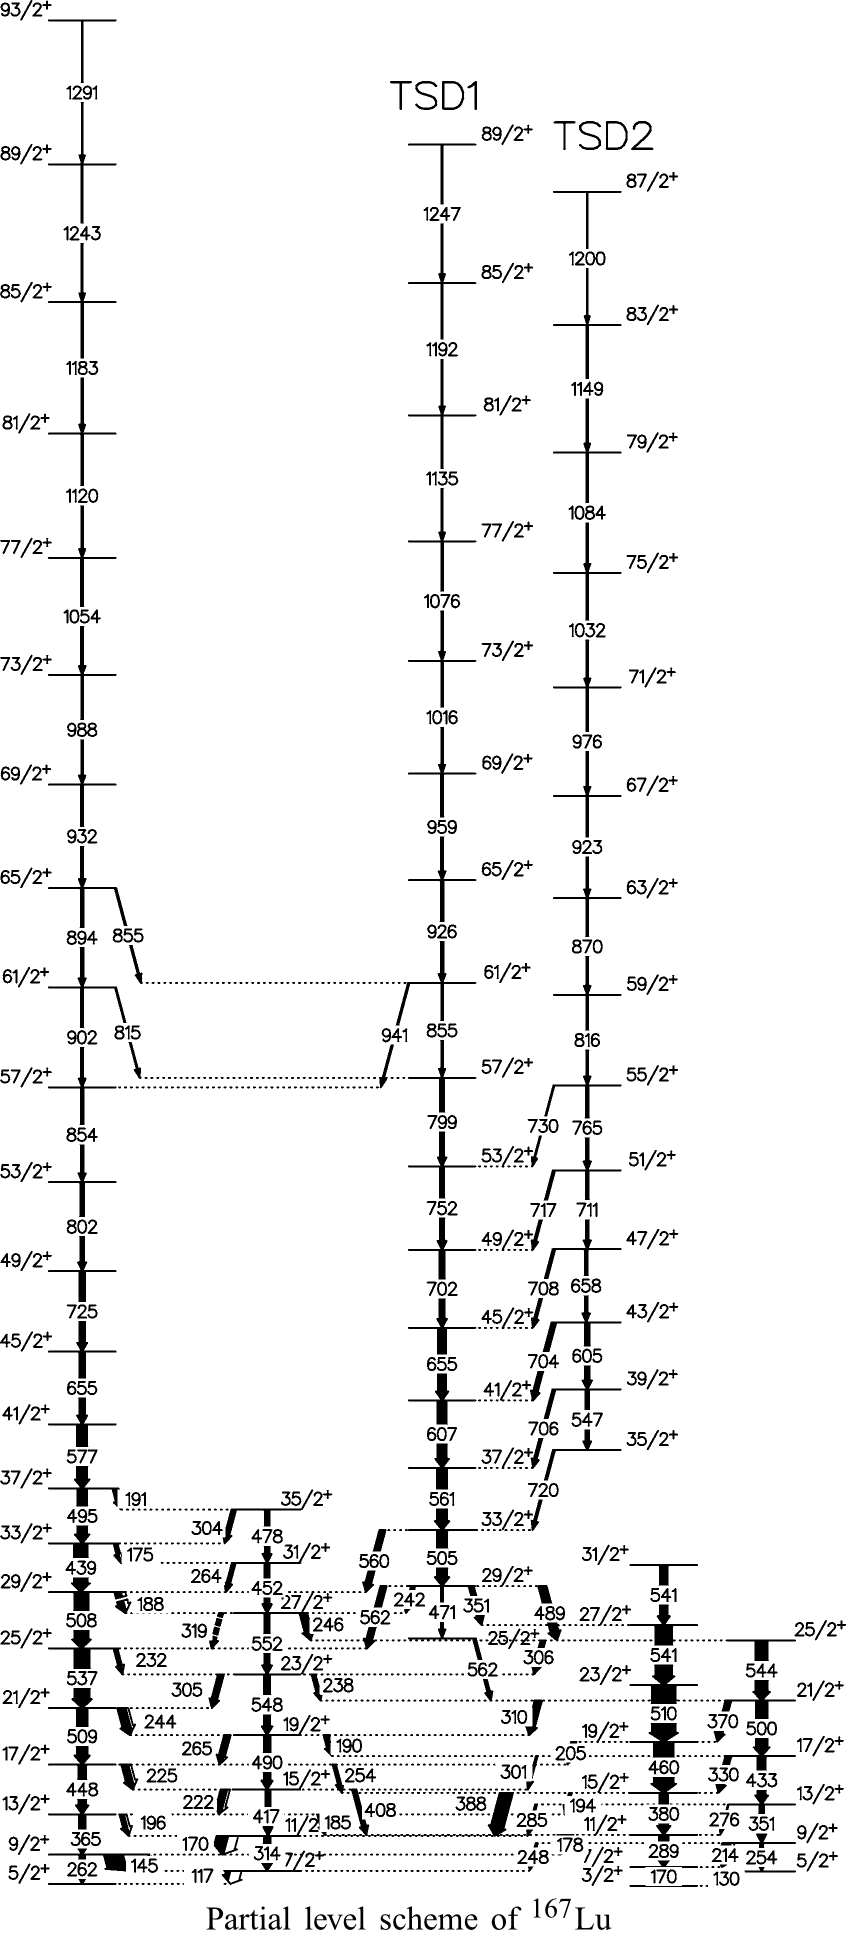
\includegraphics[width=0.4\textwidth]{./img/c1/167Lu_scheme.png}\hspace{0.1\textwidth}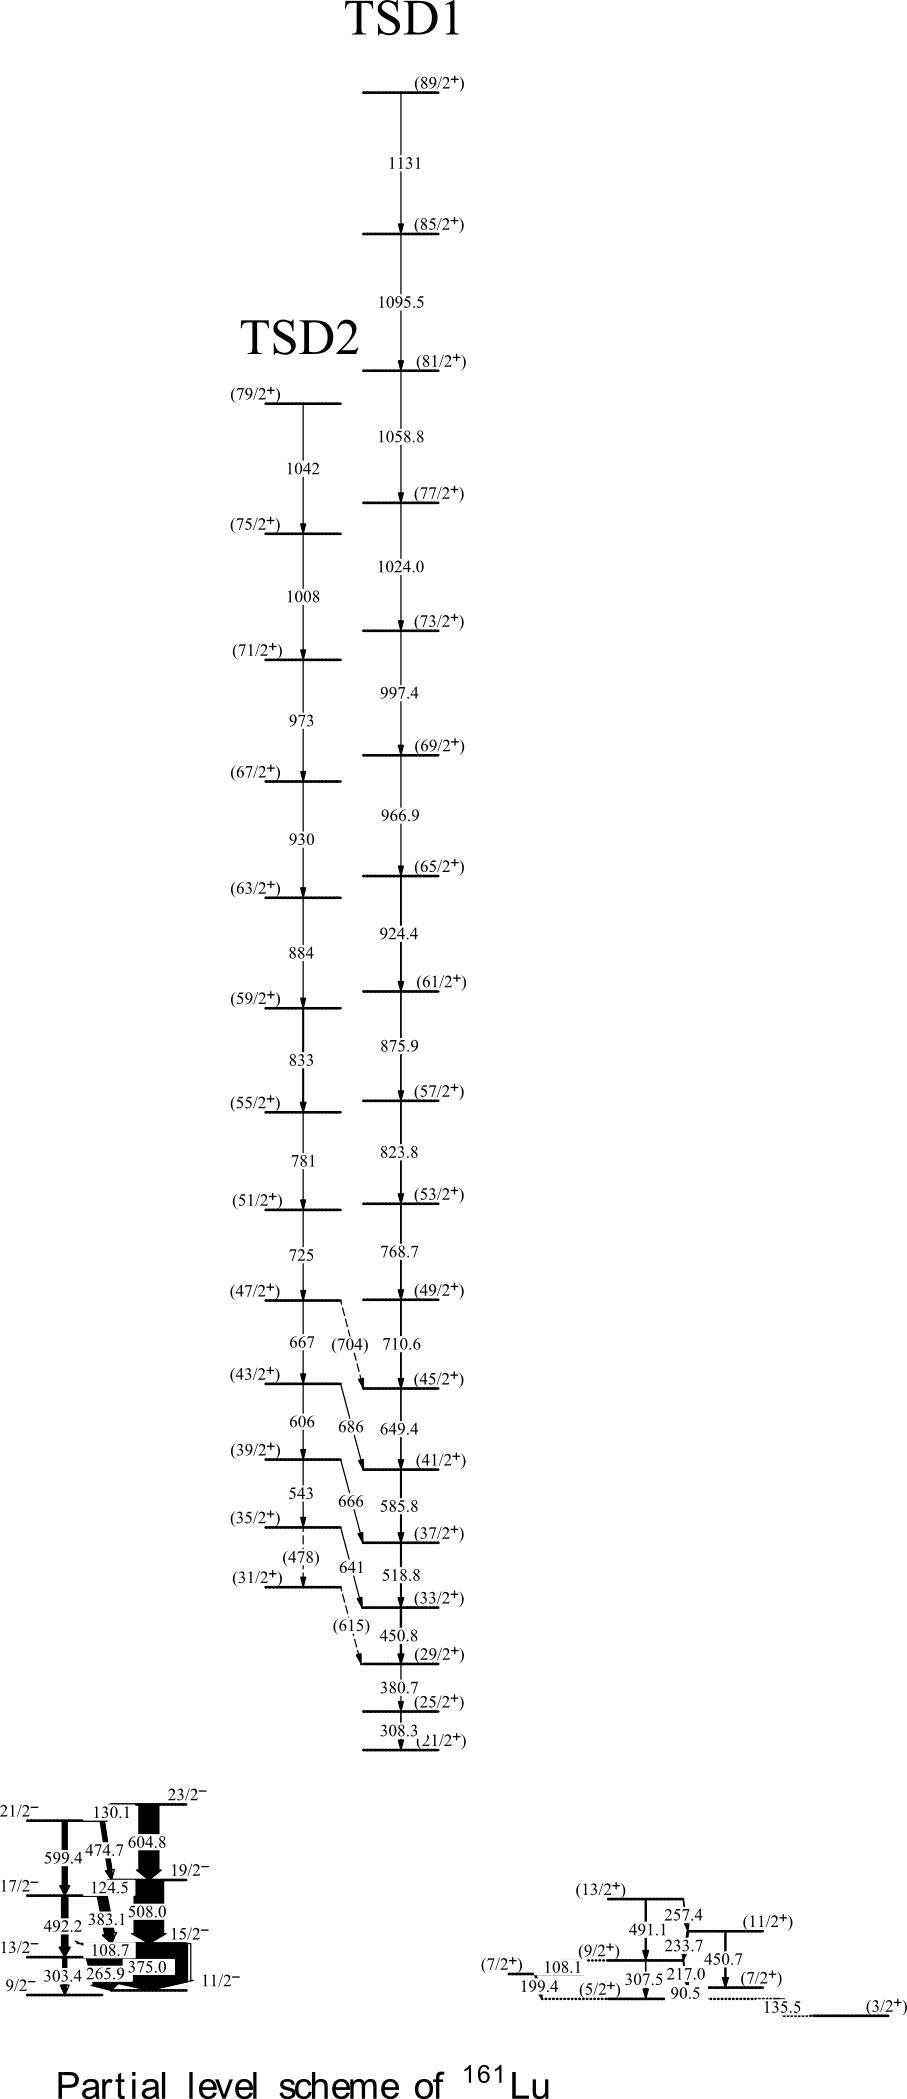
\includegraphics[width=0.4\textwidth]{./img/c1/161Lu_scheme.png}}
	\caption{Partial level schemes of $^{167}$Lu (left) and $^{161}$Lu (right). Figures adapted from Ref. \cite{wobblingIn167Lu} and Ref. \cite{wobblingIn161Lu}, respectively. In $^{167}$Lu the $n_w=0,1$ bands are labeled TSD1 and TSD2, respectively. In $^{161}$Lu the $n_w=0,1$ bands are labeled TSD1 and TSD2, respectively.\label{fig:chp1-second-wobb}}
\end{figure}

\begin{figure}[ht!]
\centerline{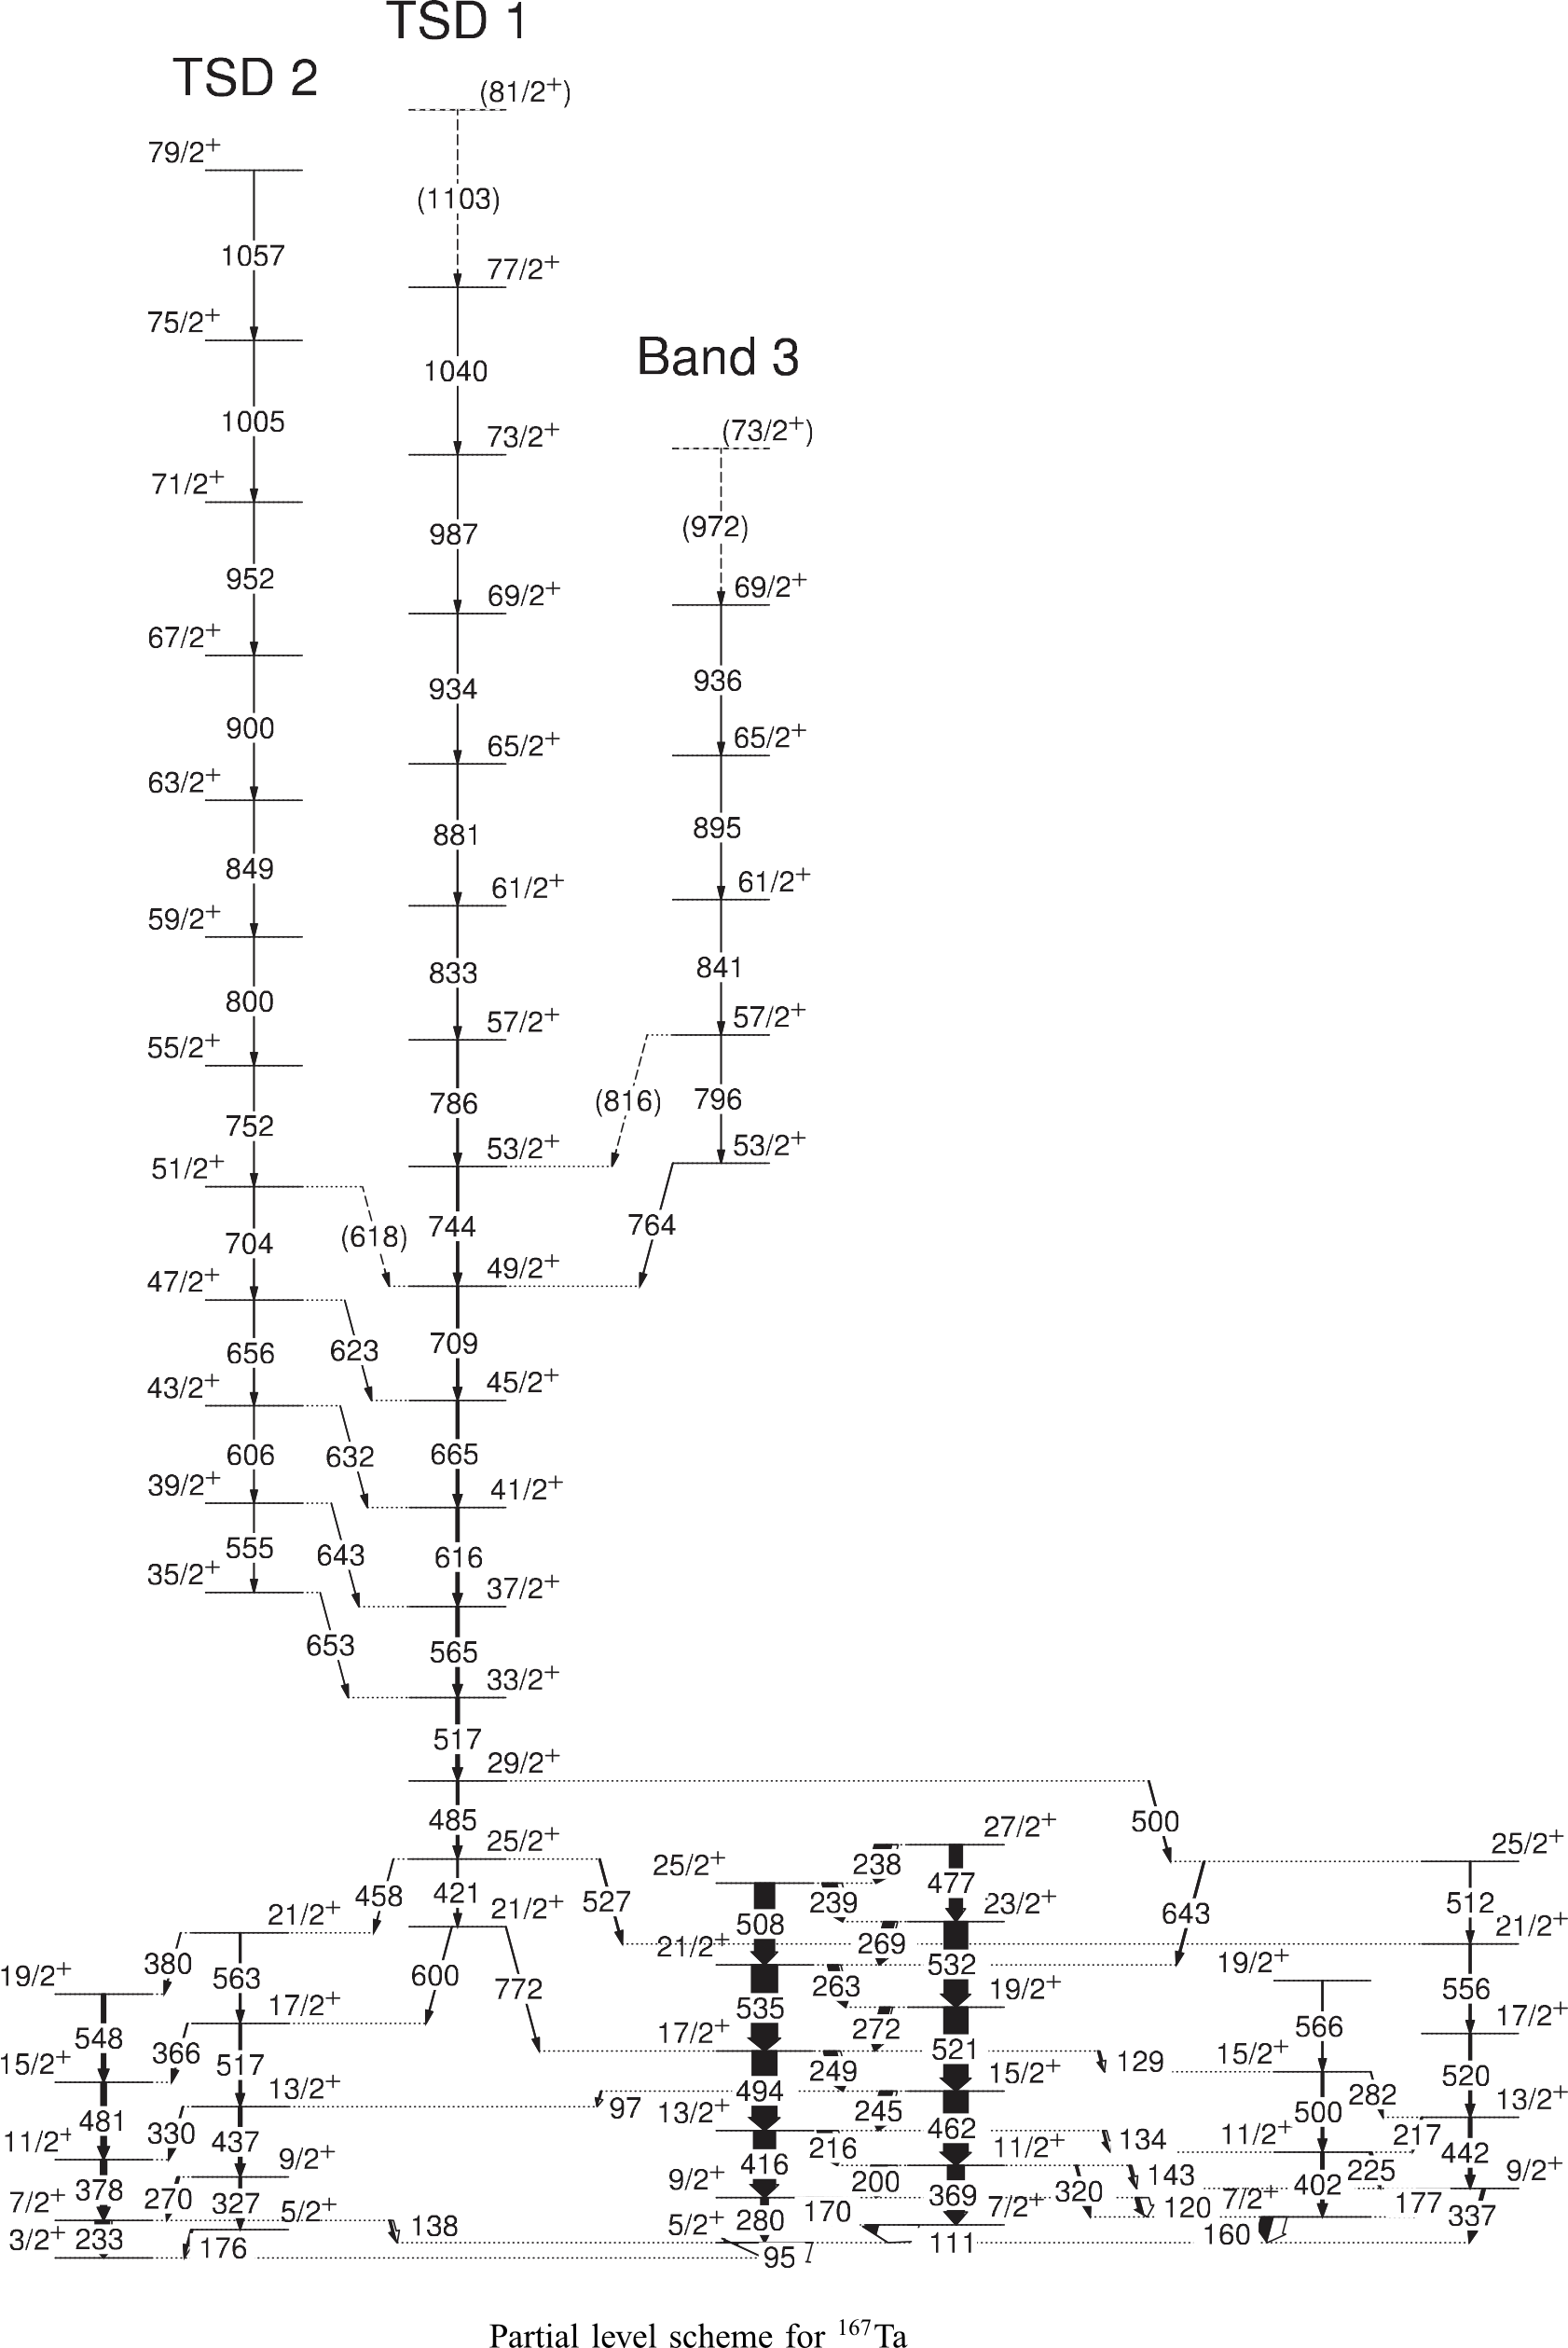
\includegraphics[width=0.6\textwidth]{./img/c1/167Ta_scheme.png}}
	\caption{Partial level scheme of $^{167}$Ta. Figure adapted from Ref. \cite{wobblingIn167Ta}. The $n_w=0,1$ bands are labeled TSD1 and TSD2, respectively.\label{fig:chp1-last-wobb}}
\end{figure}

Following the discovery of the first wobbling structure, calculations using the QTR model were used to describe the wobbling mode \cite{oldQTRWobblingTheory1,oldQTRWobblingTheory2,oldQTRWobblingTheory3,oldQTRWobblingTheory4}. Later, microscopic random phase approximation (RPA) calculations \cite{wobblingRPAMatsuzaki,wobblingRPAMatsuzaki2,wobblingRPAOi,wobblingRPAShimizu,wobblingRPAshoji} were used as well. Both theories do well in reproducing the large $B(E2)_{out}/B(E2)_{in}$ interband to intraband ratios seen in experiment. However, the QTR model, using the assumption that the odd quasiparticle aligns with the intermediate axis \cite{oldQTRWobblingTheory1,oldQTRWobblingTheory2,oldQTRWobblingTheory3,oldQTRWobblingTheory4}, fails to reproduce the experimentally observed decrease in the wobbling energy (see Fig. \ref{fig:chp1-old-wobb-freq}) which is defined by:
\begin{equation}
\label{eqn:chp4-wobb-freq}
\Delta{}E=\hbar\omega_w(I)=E(I,n_w=1)-(E(I-1,n=0)+E(I+1,n_w=0))/2
\end{equation}
In constrast the microscopic RPA calculations were able to reproduce the observed decrease in wobbling energy.
\begin{figure}[ht!]
\centerline{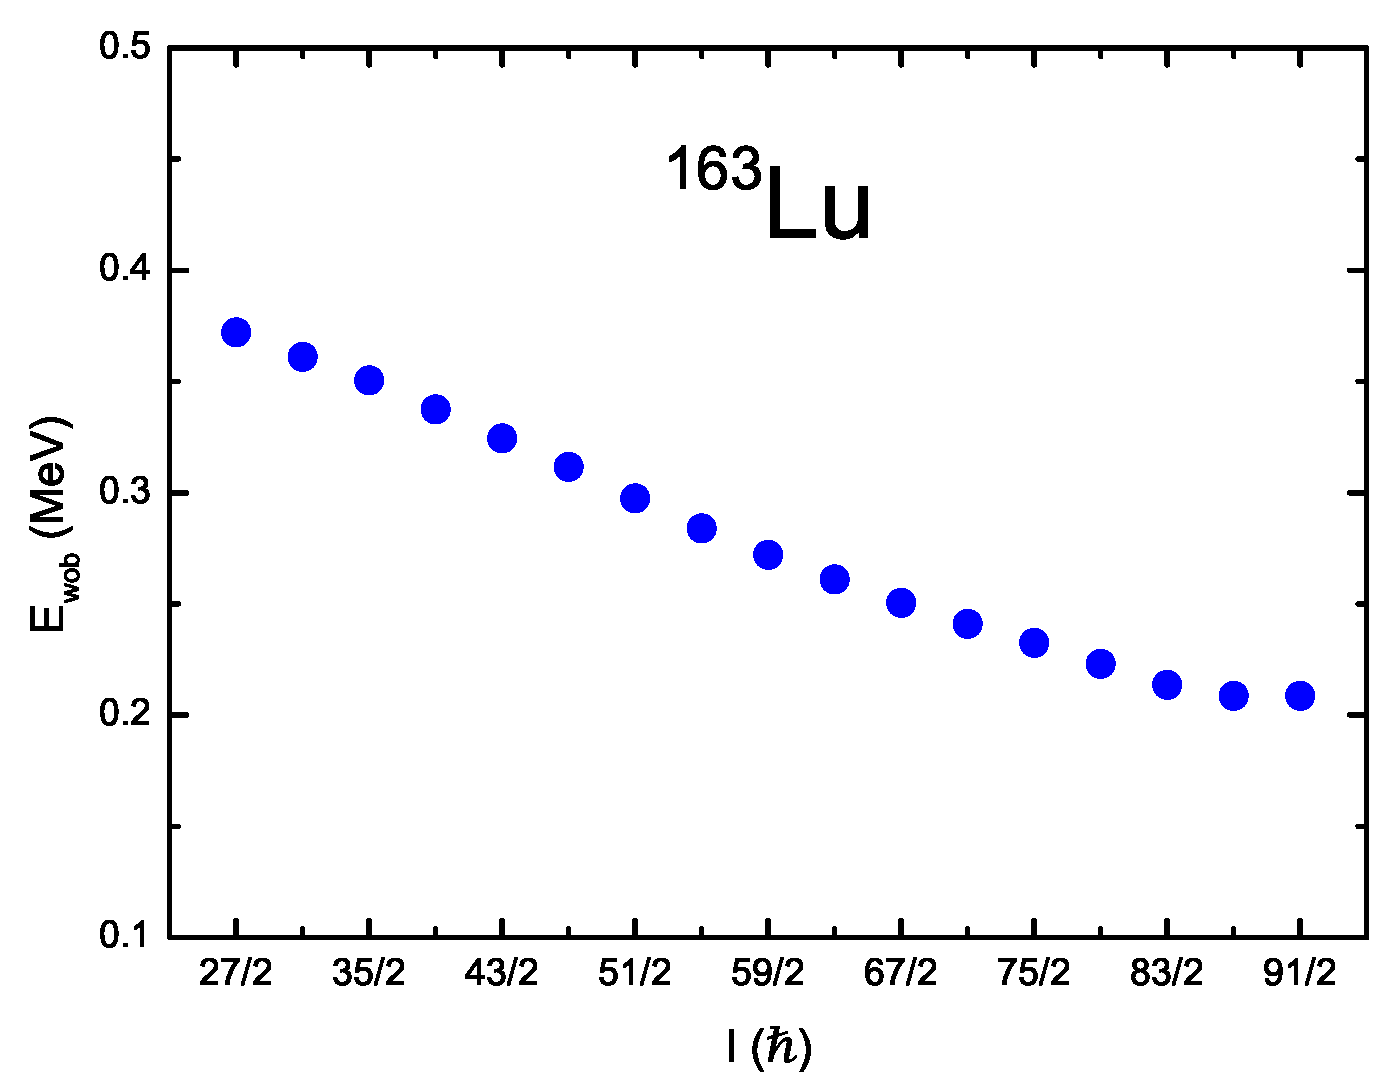
\includegraphics[height=0.25\textheight]{./img/c1/163Lu_plot.eps}\hspace{0.02\textwidth}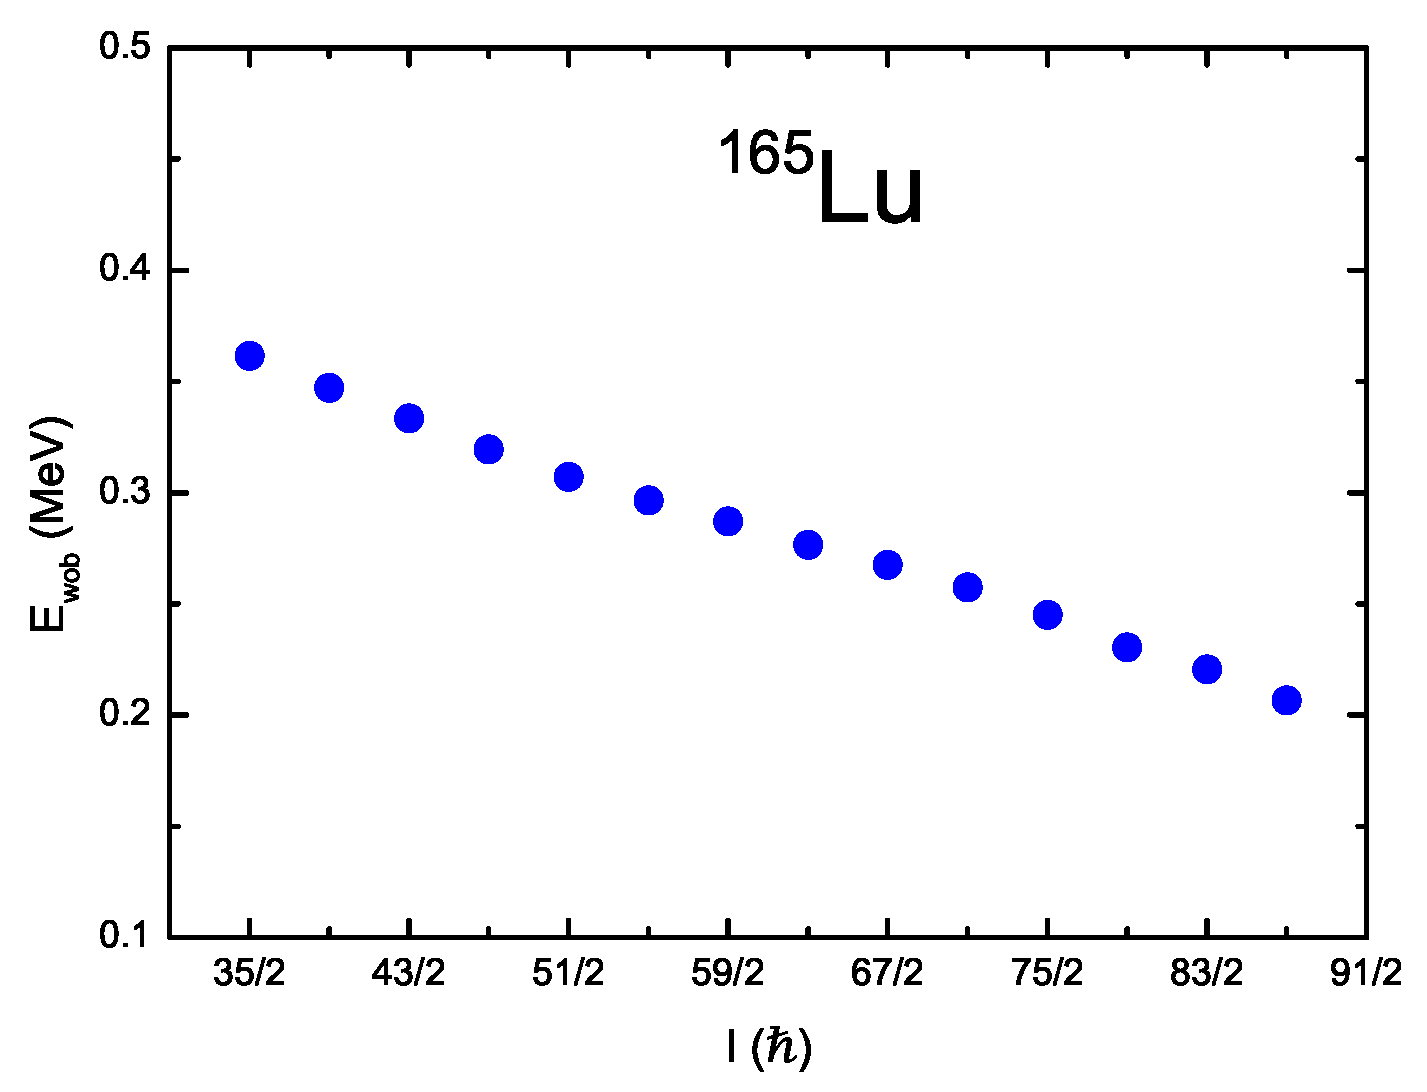
\includegraphics[height=0.25\textheight]{./img/c1/165Lu_plot.eps}}
\centerline{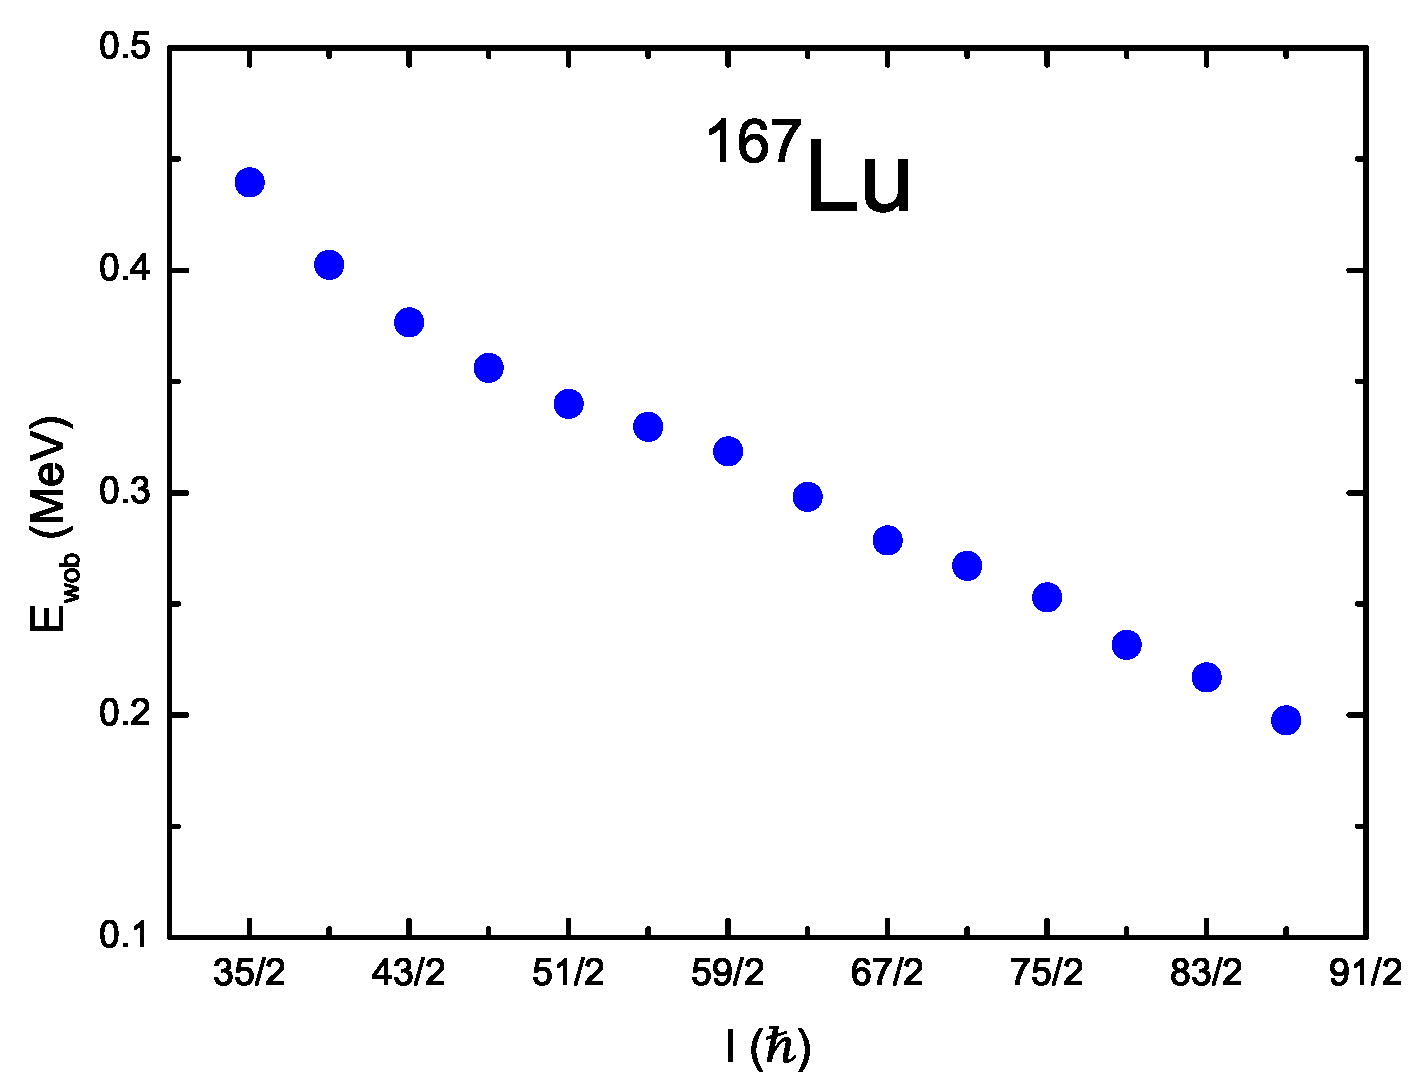
\includegraphics[height=0.25\textheight]{./img/c1/167Lu_plot.eps}\hspace{0.02\textwidth}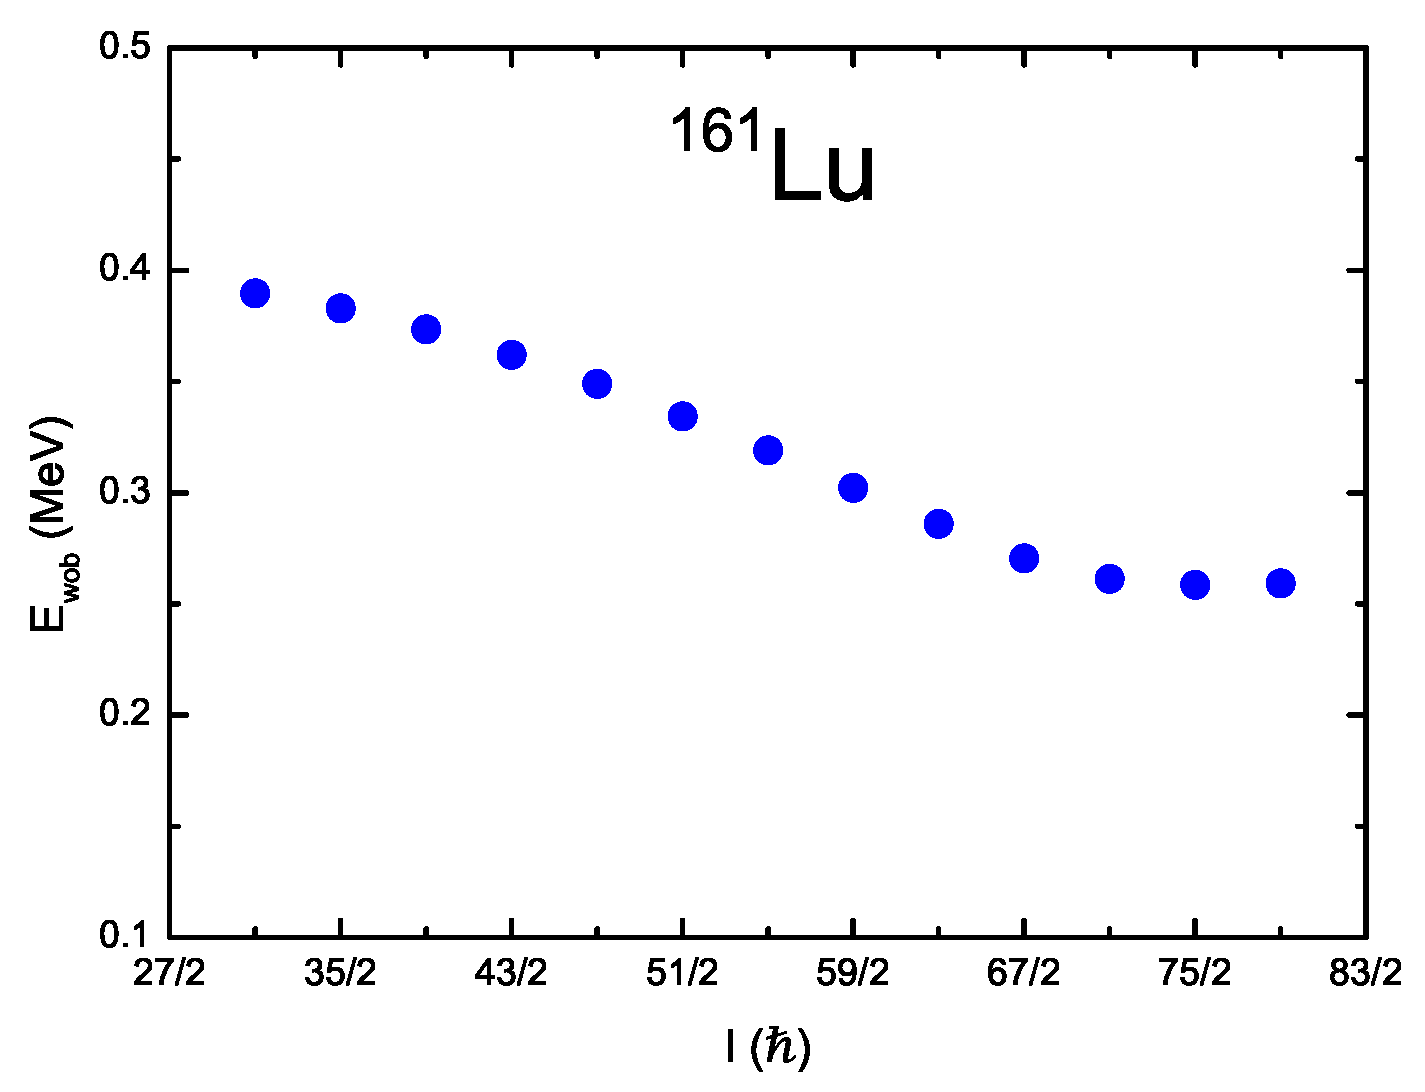
\includegraphics[height=0.25\textheight]{./img/c1/161Lu_plot.eps}}
\centerline{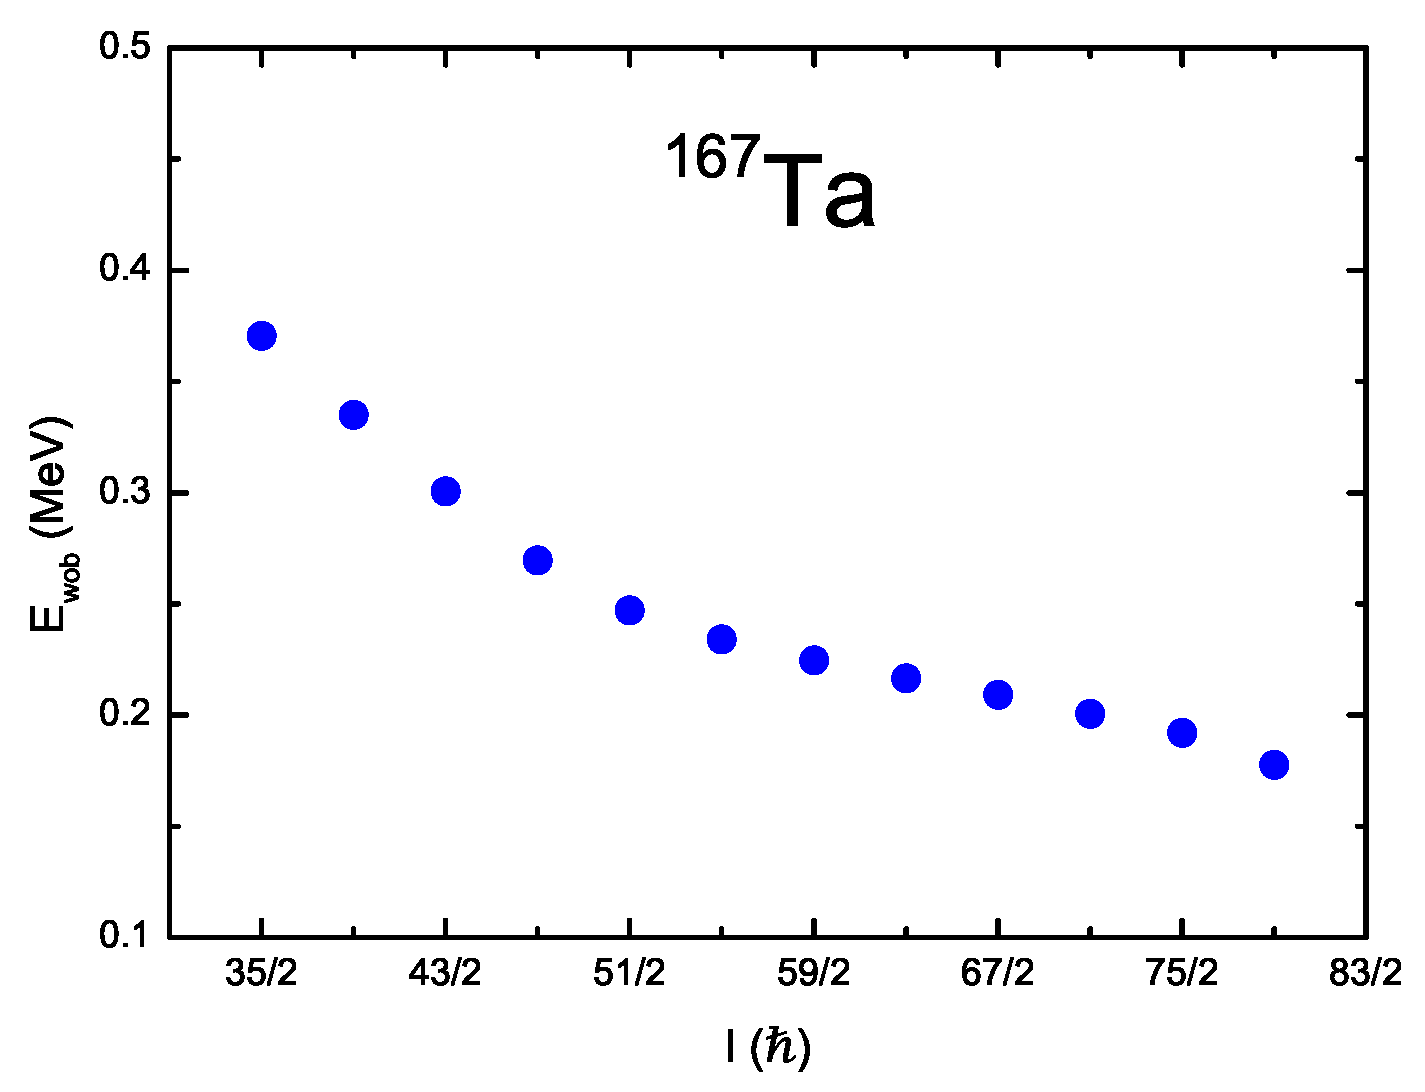
\includegraphics[height=0.25\textheight]{./img/c1/167Ta_plot.eps}}
	\caption{Wobbling frequencies of the $A\sim{}170$ wobblers. Top Left: $^{163}$Lu. Top Right: $^{165}$Lu. Middle Left: $^{167}$Lu. Middle Right: $^{161}$Lu. Bottom: $^{167}$Ta.\label{fig:chp1-old-wobb-freq}}
\end{figure}

\section{Motivation}
\label{ssec:intro-rot-motivation}
To correct the deficiency in the QTR calculations of wobbling, S. Frauendorf and F. D\"{o}nau introduced the concept of transverse and longitudinal wobbling \cite{frauendorfTransverseWobbling}. In this new scheme Refs. \cite{oldQTRWobblingTheory1,oldQTRWobblingTheory2,oldQTRWobblingTheory3,oldQTRWobblingTheory4} were describing longitudinal wobbling which is expected to have an increasing wobbling frequency. A semi-classical analysis of transverse wobbling, which has the quasiparticle couple to an axis perpendicular to the intermediate axis, shows that the modified mode exhibits a decreasing wobbling frequency as has been seen in experimental observations of wobbling while reproducing the interband to intraband $B(E2)$ ratios.

The work presented in this dissertation was performed to test the theory of transverse wobbling and show that the $A\sim{}130$ region is a viable place to search for the wobbling modes in nuclei. Toward that end, a suspected transverse wobbling was measured in \pr{} and its transverse wobbling nature was confirmed by showing that interband $n_w=1\rightarrow{}n_w=0$ transitions had $\Delta{}I=1, E2$ nature using angular distribution and polarization asymmetry measurements. Finally, theoretical work in the framework of the QTR and TAC models was performed; thus confirming that the wobbling mode is well described by the QTR framework.
